
Na área-base de 500 $\times$ 500 m (Figura~\ref{fig:pdr}), o PDR médio cai
de 85,2\%, 81,0\% e 78,6\% a 1 m/s para 66,3\%, 32,8\% e 36,4\% a 20 m/s, respectivamente para AODV,
OLSR e DSDV. A vazão acompanha a entrega porque a demanda é fixa.
O comportamento é compatível com a dificuldade de manter rotas sob mobilidade,
mas as métricas agregadas não separam perdas por ausência de caminhos,
desatualização de rotas e contenção no canal.

\begin{figure}[ht]
\centering
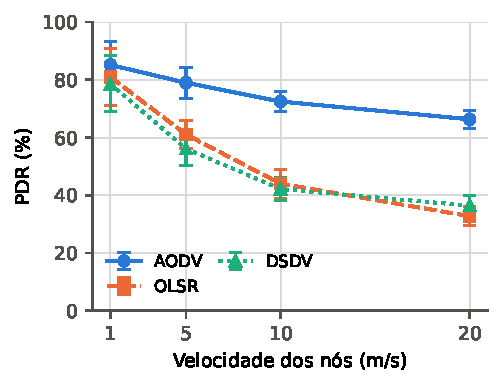
\includegraphics[width=.42\textwidth]{area-500m/pdr-vs-velocidade}
\hfill
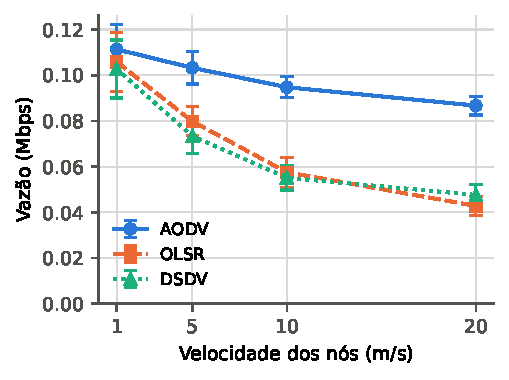
\includegraphics[width=.42\textwidth]{area-500m/vazao-vs-velocidade}
\caption{PDR e vazão no cenário-base (média e IC de 95\%, 20 runs).}
\label{fig:pdr}
\end{figure}

O atraso médio do AODV passa de 14,8 para 137,4 ms entre 1 e
20 m/s. A 20 m/s, OLSR e DSDV apresentam 15,7 e 12,0 ms, com menor entrega.
Atraso e jitter (Figura~\ref{fig:atraso}) devem ser lidos com o PDR:
os pacotes perdidos não entram nas médias e o descarte de trajetos difíceis
pode favorecer artificialmente a leitura de latência. Não se conclui
superioridade geral de um protocolo a partir de uma única métrica.

\begin{figure}[ht]
\centering
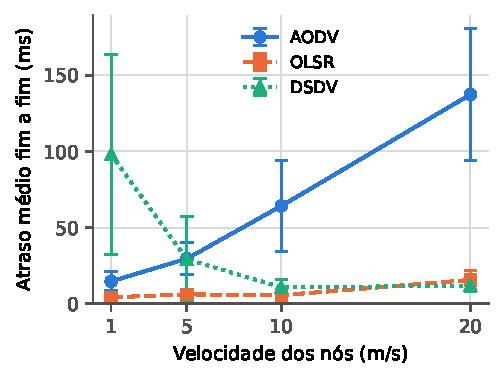
\includegraphics[width=.42\textwidth]{area-500m/atraso-vs-velocidade}
\hfill
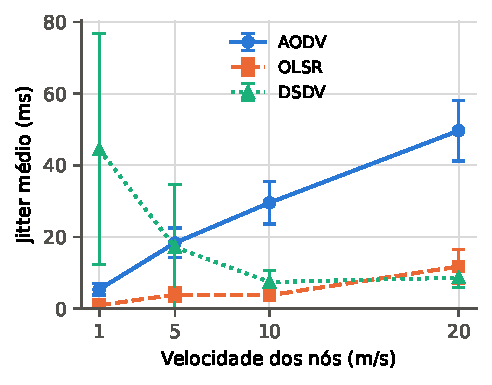
\includegraphics[width=.42\textwidth]{area-500m/jitter-vs-velocidade}
\caption{Atraso e jitter no cenário-base (média e IC de 95\%).}
\label{fig:atraso}
\end{figure}

A Figura~\ref{fig:comparativo} resume o base a 10 m/s: os PDRs são
72,5\%, 44,0\% e 42,2\%, na ordem AODV, OLSR e DSDV. As médias entre runs dos saltos dos
pacotes entregues são 2,3; 1,7; 1,7, confirmando encaminhamento por múltiplos
saltos em parte das entregas. Isso não estima a conectividade dos pares
que não entregaram pacotes.

\begin{figure}[ht]
\centering
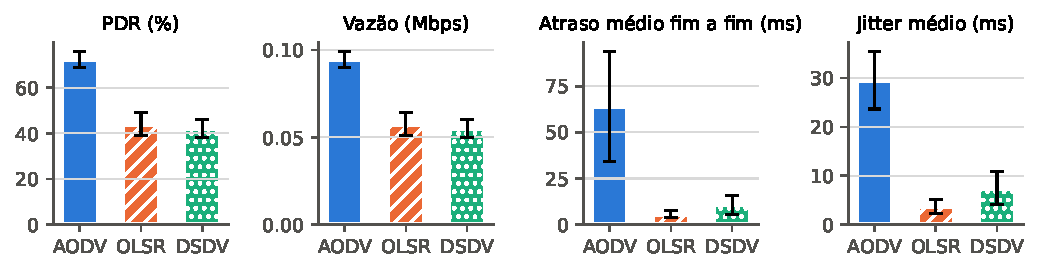
\includegraphics[width=.92\textwidth]{area-500m/comparativo-10ms}
\caption{Comparação dos protocolos a 10 m/s no base (média e IC de 95\%).}
\label{fig:comparativo}
\end{figure}

A variável adicional altera a entrega sem modificar o rádio
(Figura~\ref{fig:area}). A 20 m/s, o PDR médio em 300 $\times$ 300 m é
87,2\%, 67,0\% e 67,7\%, enquanto em 700 $\times$ 700 m é 37,3\%, 14,4\% e 18,0\%, na mesma ordem
de protocolos. A redução de densidade e o aumento de distâncias são
compatíveis com essa degradação. Não se atribui o resultado a prédios ou
árvores específicos: o ambiente é representado apenas pelo expoente fixo.
Os ICs mostram a dispersão entre runs; não se realizou teste de hipótese
para declarar diferenças estatisticamente significativas entre protocolos.
Em 700 $\times$ 700 m, o PDR médio do AODV sobe de 35,5\% a 1 m/s
para 52,2\% a 5 m/s, antes de cair: a tendência do base não é universal.
O possível efeito de novos encontros e do transiente de mobilidade não foi
isolado por medidas de conectividade temporal.

\begin{figure}[ht]
\centering
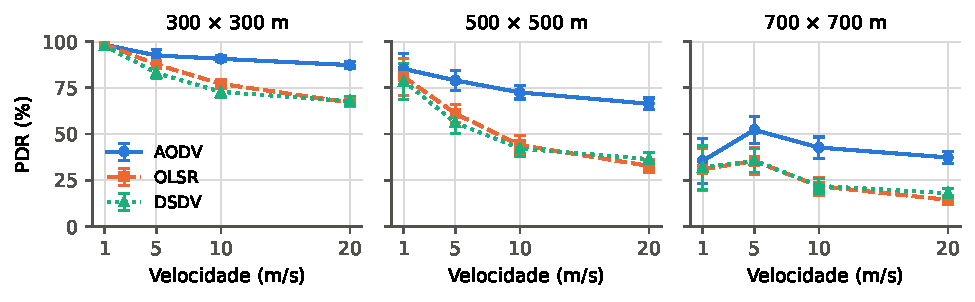
\includegraphics[width=.9\textwidth]{area/pdr-por-area}
\caption{PDR por velocidade nas três áreas, com rádio e canal de propagação
fixos (média e IC de 95\%).}
\label{fig:area}
\end{figure}
